\chapter{Cronograma}
\label{cap:cronograma}

Este capítulo apresenta o planejamento temporal das atividades desenvolvidas no TCC 1 e planejadas para o TCC 2, organizadas em fases sequenciais ao longo dos semestres letivos.

\section{Cronograma do TCC 1}

O TCC 1, desenvolvido no período de setembro a dezembro de 2025, concentrou-se na fundamentação teórica, coleta e análise exploratória dos dados. A Figura~\ref{fig:cronograma_tcc1} apresenta a distribuição temporal das atividades executadas, organizadas em cinco fases principais: (1) Planejamento da Pesquisa, (2) Coleta de Dados, (3) Análise dos Dados, (4) Metodologia e (5) Relatório.

\begin{figure}[htb]
	\centering
	\caption{Cronograma executado no TCC 1 (setembro a dezembro de 2025)}
	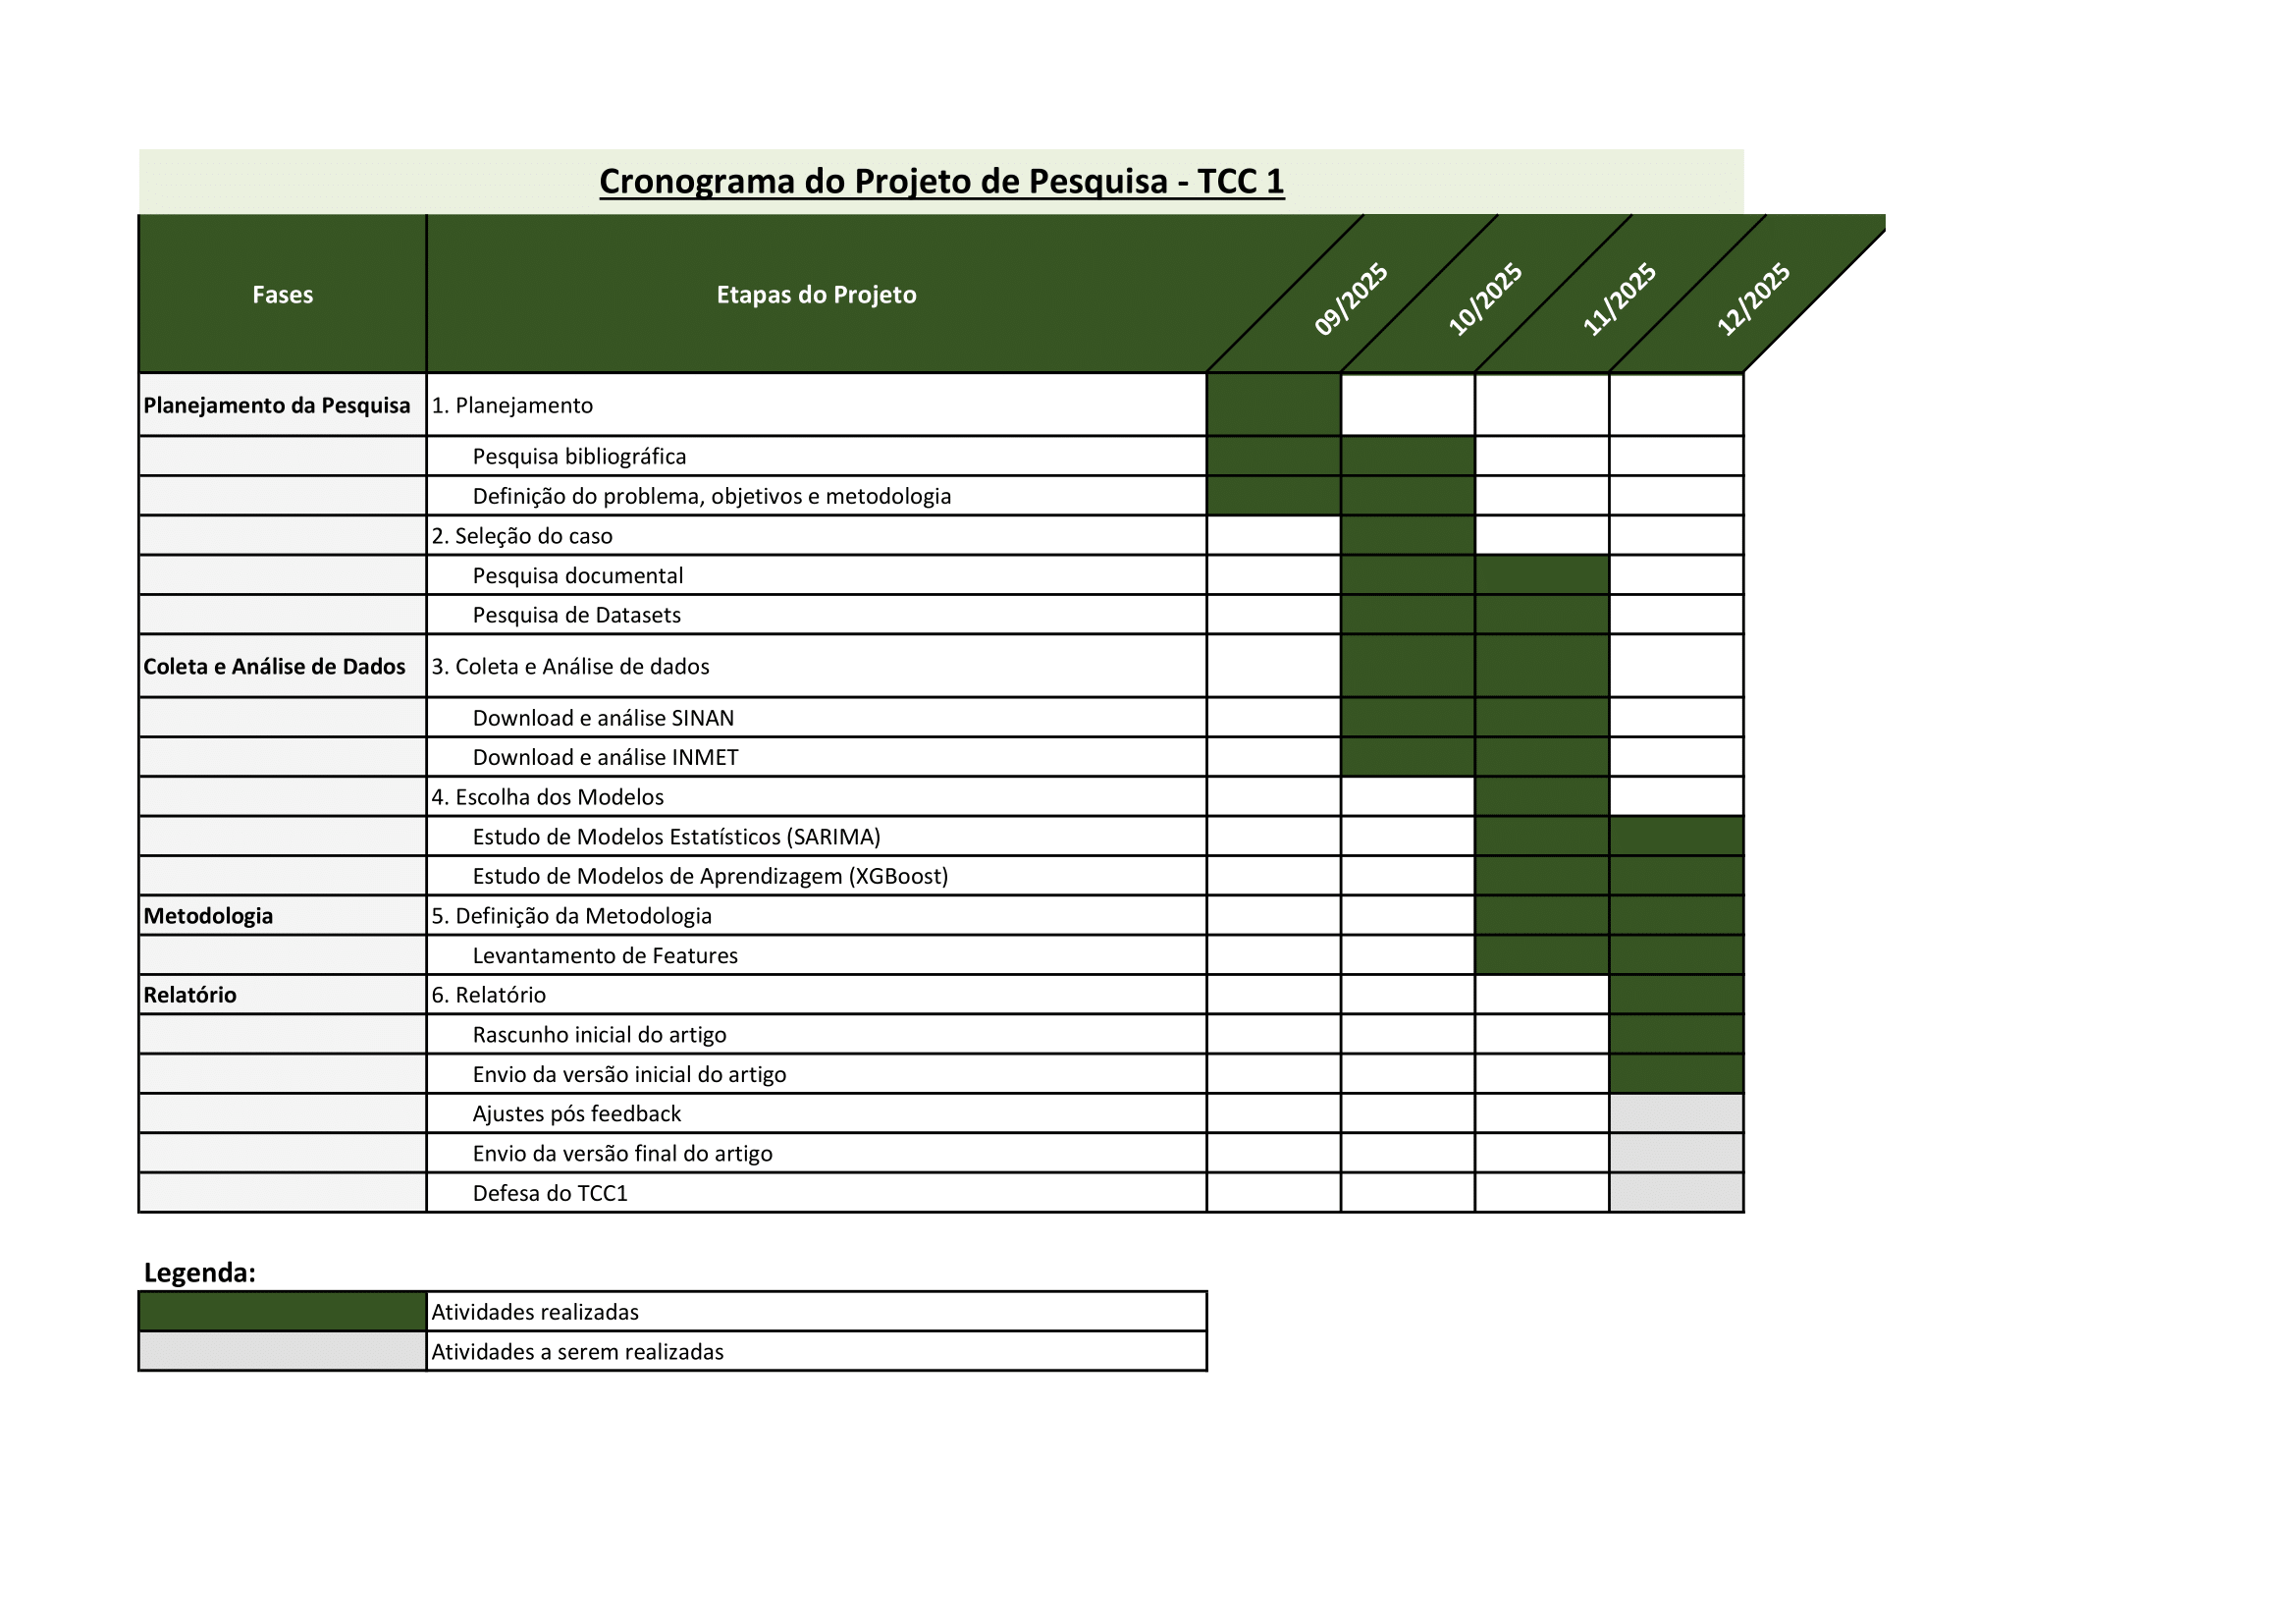
\includegraphics[width=\textwidth]{../Cronogramas/Cronograma_TCC1_2025-1.png}
	\label{fig:cronograma_tcc1}
	\fonte{Elaborado pelo autor.}
\end{figure}

As atividades realizadas incluíram a revisão bibliográfica sobre epidemiologia da dengue e modelos preditivos, a identificação e caracterização das bases de dados (SINAN e INMET), o desenvolvimento do pipeline de engenharia de dados com scripts de coleta automatizada, a análise estatística exploratória com cálculo de correlações e testes de causalidade de Granger, e a redação dos capítulos iniciais do trabalho.

\section{Cronograma do TCC 2}

O TCC 2, planejado para o período de janeiro a março de 2026, focará no desenvolvimento, treinamento e validação dos modelos preditivos, além da implementação de um sistema de alerta automatizado. A Figura~\ref{fig:cronograma_tcc2} apresenta a distribuição temporal das atividades previstas, organizadas em seis fases: (1) Feature Engineering, (2) Modelos Baseline (SARIMA/Prophet), (3) Machine Learning (Random Forest/XGBoost), (4) Deep Learning (LSTM/BiLSTM), (5) Validação e Comparação, e (6) Redação Final.

\begin{figure}[htb]
	\centering
	\caption{Cronograma planejado para o TCC 2 (janeiro a março de 2026)}
	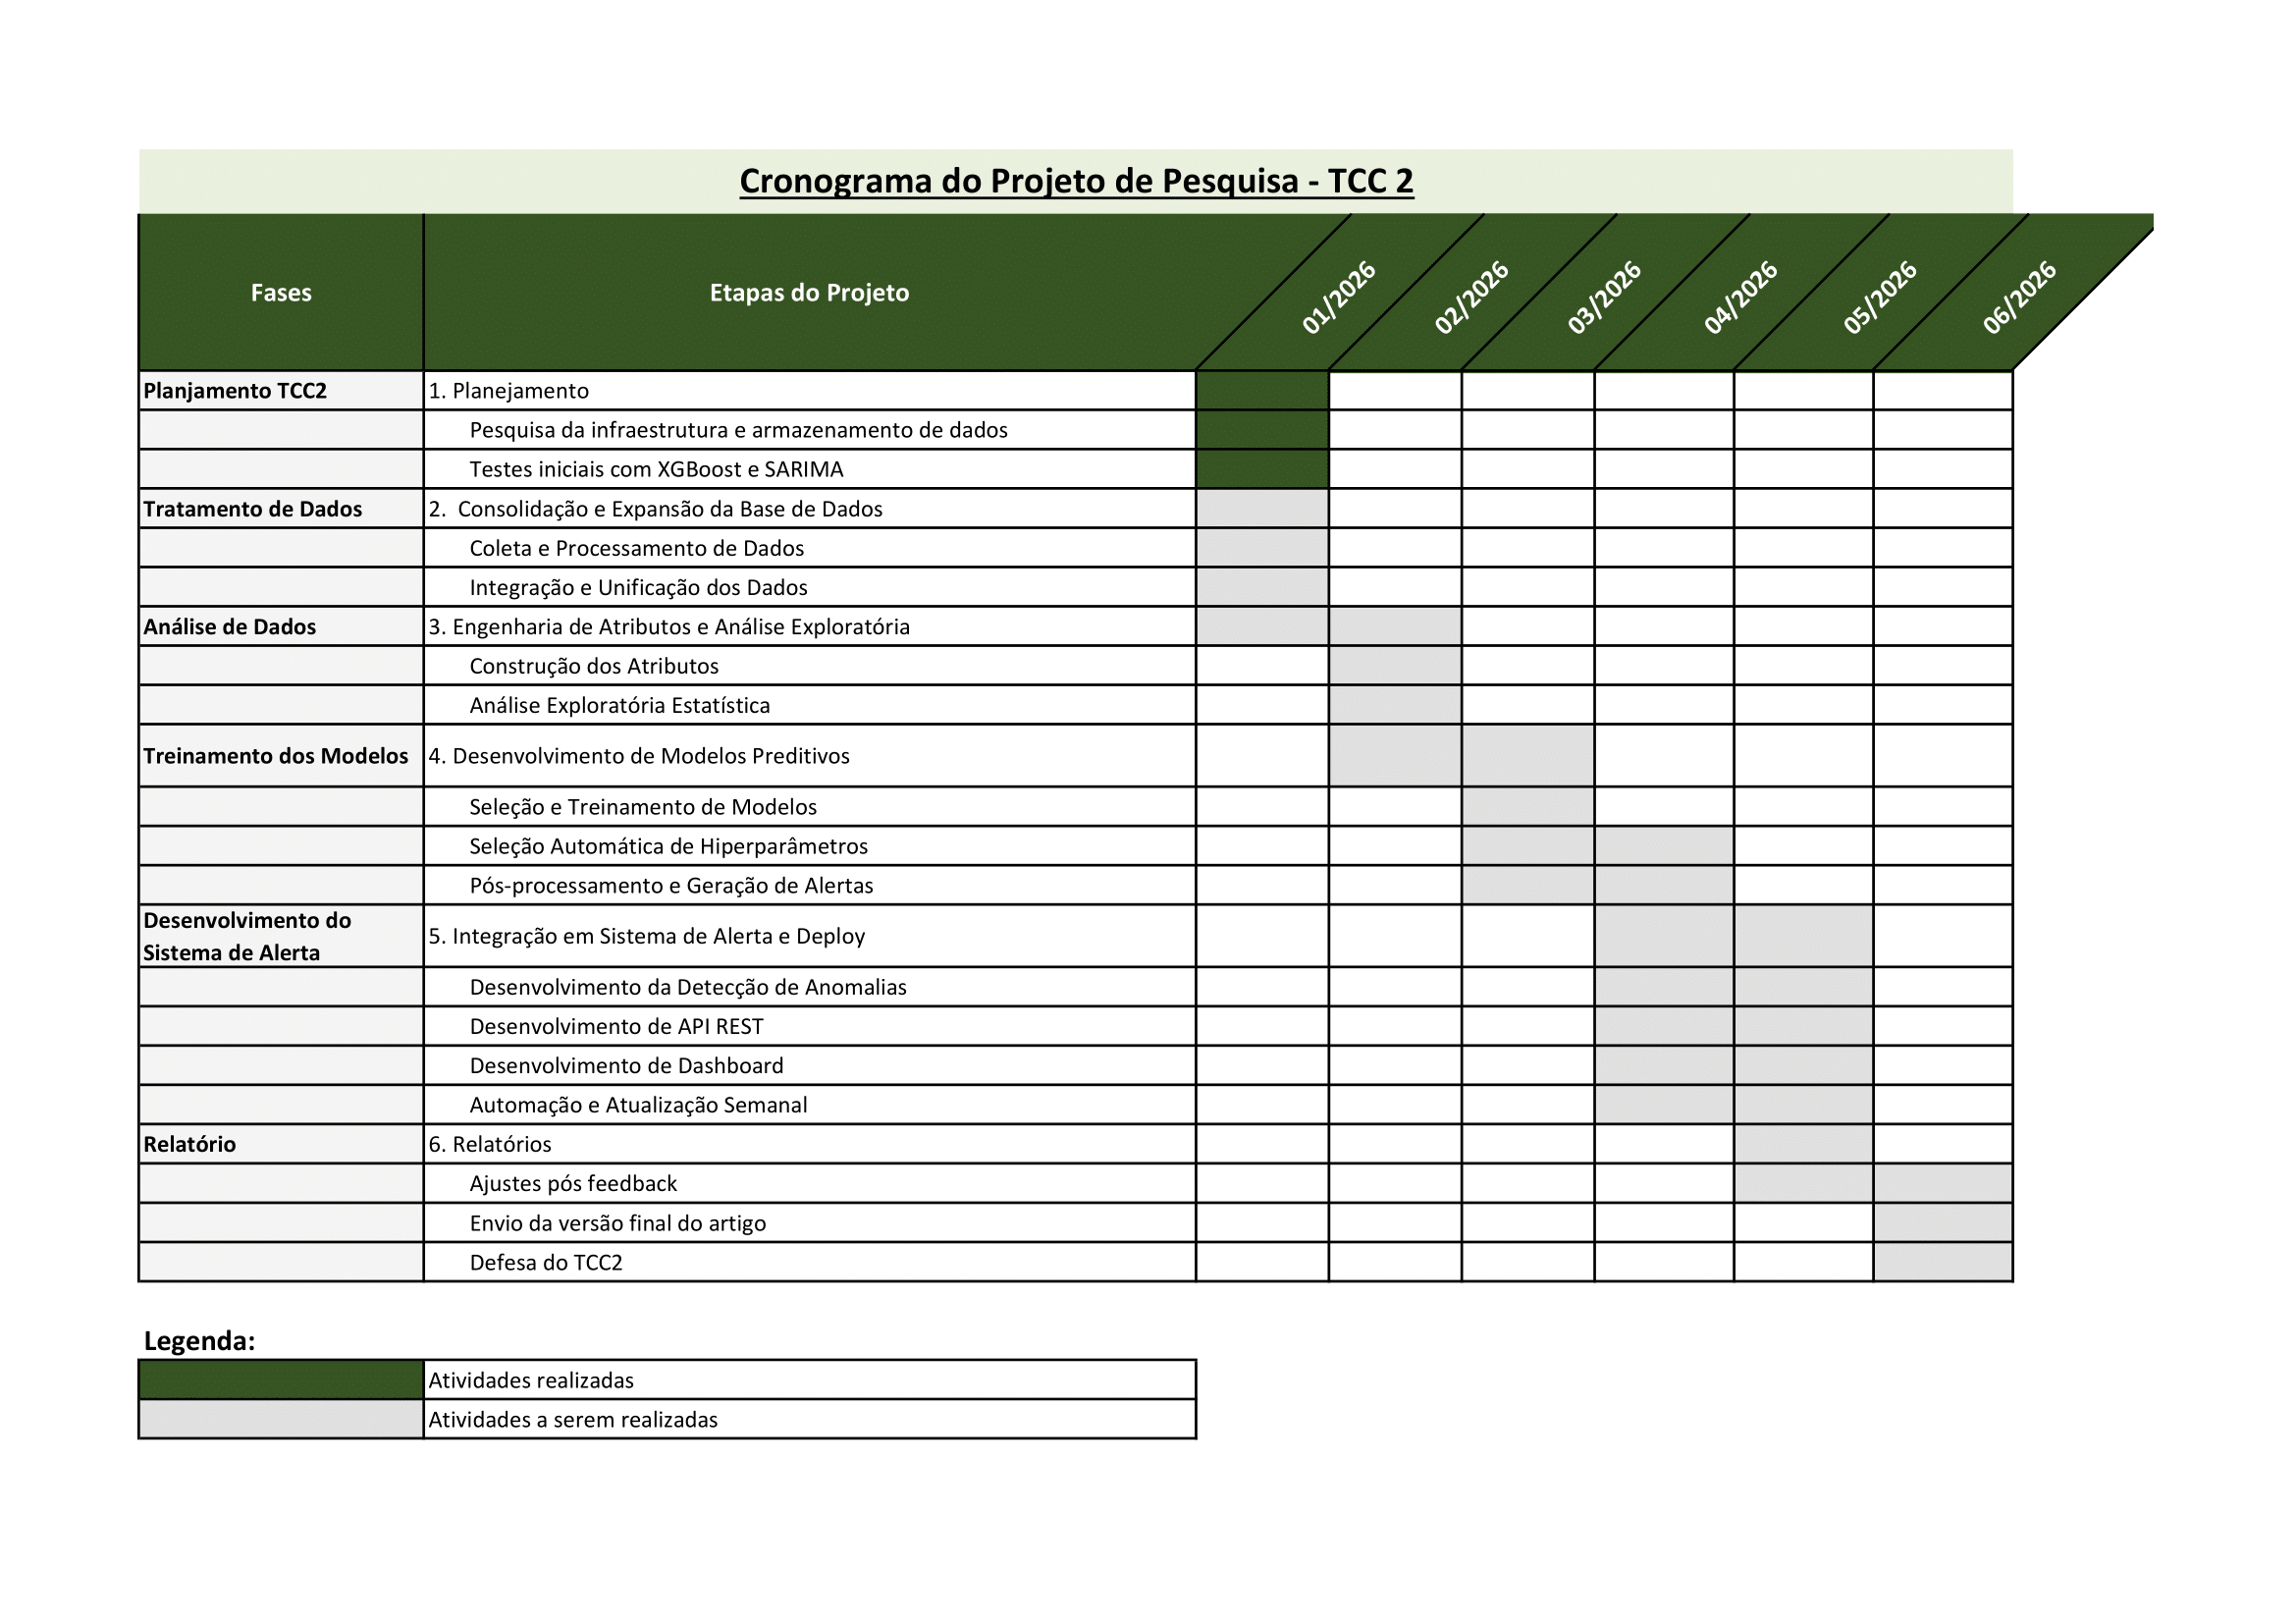
\includegraphics[width=\textwidth]{../Cronogramas/Cronograma_TCC2_2026-1.png}
	\label{fig:cronograma_tcc2}
	\fonte{Elaborado pelo autor.}
\end{figure}

As atividades planejadas incluem a engenharia de atributos com criação de lags temporais e variáveis derivadas, a implementação de modelos estatísticos (SARIMA/SARIMAX e Prophet) como baseline, o desenvolvimento de modelos de machine learning (Random Forest e XGBoost) com otimização de hiperparâmetros, a implementação de arquiteturas de deep learning (LSTM, BiLSTM e CNN-LSTM), a validação rigorosa com walk-forward validation e comparação estatística entre modelos, e a redação final do trabalho com preparação da defesa.

\section{Considerações sobre o Planejamento}

O projeto está estruturado em aproximadamente 30 semanas de trabalho, distribuídas entre dois semestres letivos. O TCC 1 (14 semanas) estabeleceu a base conceitual e metodológica do trabalho, enquanto o TCC 2 (16 semanas) dedicar-se-á à implementação prática e avaliação dos modelos. As Figuras~\ref{fig:cronograma_tcc1} e~\ref{fig:cronograma_tcc2} evidenciam a progressão lógica das atividades, respeitando as dependências metodológicas entre as etapas e considerando a carga horária acadêmica do estudante.
